\section{Representación de los datos }
\label{sec:cap2-tecnicas-graficas-representacion}
Los objetos del mundo real se pueden describir mediante los fenómenos discretos y continuos, donde las variables y objetos se muestrean y organizan para lograr una representación adecuada. En un
SIG existen básicamente dos modelos lógicos que se conocen como formato raster y formato vectorial
y que dan lugar a los dos grandes tipos de capas de información espacial \citep{fAlonsoSig2006}.

\subsection{Formato raster}
El formato raster se centra en las propiedades del espacio más que en la precisión de la
localización. Divide el espacio en un conjunto regular de celdas, donde cada una contiene un
número que puede ser el identificador de un objeto o del valor de una variable
\citep{fAlonsoSig2006}. Se trata de un modelo de datos muy adecuado para la representación de
variables continuas en el espacio.

Los datos raster se encuentran definidas como una grilla con un número determinado de filas y
columnas, donde a celda se le asocia un único valor. Los datos raster pueden ser imágenes, donde
el valor asociado a cada celda o píxel de la imagen, representa un color. Otros valores
registrados para cada celda puede ser un valor discreto o un valor nulo para indicar que no se
disponen datos.

\begin{figure}[H]
\centering
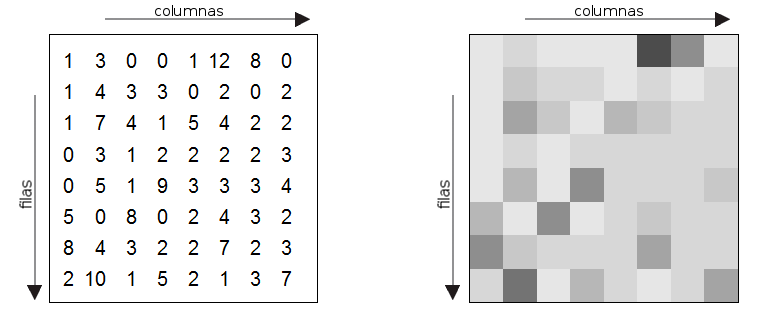
\includegraphics[width=0.9\textwidth]{capitulo-2/graphics/representacion-raster.png}
\caption{\label{fig:sig-capa-raster} Comparación entre la definición de una capa raster y su representación. }
\end{figure}

La resolución y la nitidez del la capa raster depende del tamaño de la celda, donde el tamaño esta
asociado a la cantidad de columnas y filas de la capa raster. Mientras más filas y columnas cuente
una capa raster, más nítida será la imagen resultante.

\subsection{Formato vectorial}
Los datos vectoriales, se caracterizan por la precisión de localización de los elementos
geográficos en el espacio, donde los fenómenos a representar son discretos, con límites bien
definidos. Generalmente se considera que el formato vectorial es más adecuado para la
representación de entidades o variables cualitativas y el formato raster para representar
superficies\citep{fAlonsoSig2006}.

Los diferentes objetos, vectoriales, se encuentran representados como puntos, lineas o polígonos
\citep{fAlonsoSig2006}. De tal forma que para modelar digitalmente las entidades del mundo real se
utilizan estos tres elementos geométricos.

\begin{figure}
\centering
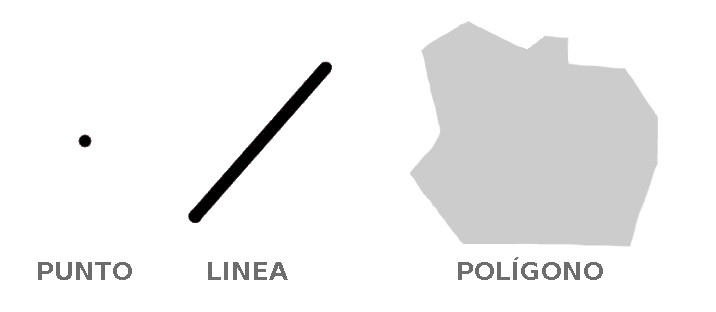
\includegraphics[width=0.8\textwidth]{capitulo-2/graphics/dimensiones-datos.jpg}
\caption{\label{fig:sig-xyz} Elementos geométricos utilizados para modelar digitalmente las entidades en un SIG.}
\end{figure}

\begin{itemize}
    \item \textit{Puntos} : se utilizan para representar las entidades geográficas que pueden ser
    descritas como un fenómeno puntual. Estos transmiten la menor cantidad de información y su representación es la más simple.

    \item \textit{Líneas o polilíneas} : las líneas unidimensionales o polilíneas son usadas para
    representar elementos con rasgos lineales como ríos, caminos, ferrocarriles, rastros, líneas
    topográficas o curvas de nivel.

    \item \textit{Polígonos} : se utilizan para representar elementos geográficos que cubren un
    área particular de la superficie de la tierra. Los polígonos transmiten mayor cantidad de
    información y en ellos se pueden medir el perímetro y el área.
\end{itemize}

\subsection{Ventajas y desventajas de los formatos raster y vectorial}

El debate acerca de la conveniencia de uno u otro modelo debe basarse en el tipo de estudio o
enfoque que se quiera hacer, pero también del software y fuentes de datos disponibles
\citep{fAlonsoSig2006}.

El formato raster se considera el más adecuado para representar eficientemente las superficies.
Estas solo pueden representarse vectorialmente mediante modelos híbridos que no resultan adecuados
para la realización de posteriores análisis ya que todas las operaciones que permite el modelo
ráster resultaran mucho más lentas con el modelo vectorial \citep{fAlonsoSig2006}.
Tradicionalmente se ha considerado que para la representación de los objetos resulta más eficiente
la utilización de un formato vectorial ya que la estructura de los datos es compacta y almacena
los datos sólo de los elementos digitalizados por lo que requiere menos memoria para su
almacenamiento y tratamiento \citep{fAlonsoSig2006}. Los gráficos vectoriales, se caracterizan por
no perder la definición a media que se aumenta la escala para la visualización.


\begin{figure}[H]
\begin{minipage}{\textwidth}
    \begin{tabular}{c c }
        \initbox
        \num\putindeepbox[7pt]{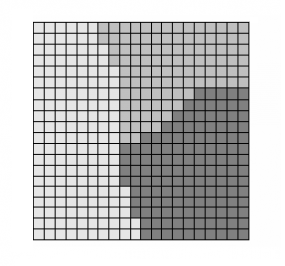
\includegraphics[width=0.4\textwidth]{capitulo-2/graphics/formato-raster.png}} &
        \num\putindeepbox[7pt]{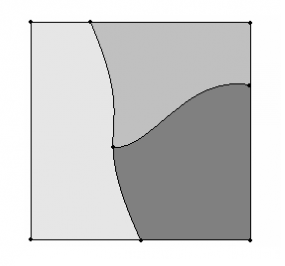
\includegraphics[width=0.4\textwidth]{capitulo-2/graphics/formato-vectorial.png}} \\
    \end{tabular}
    \caption{\label{fig:sig-raster-vs-vectorial} Representación de una misma superficie, mediante los formatos ráster y vectorial, en un SIG.}

    \footnotetext[1]{Formato Ráster.}
    \footnotetext[2]{Formtao Vectorial.}
\end{minipage}
\end{figure}


En general las ventajas del modelo ráster radican en, su simplicidad y la velocidad de ejecución de
los operadores lo que lo convierte en el modelo a utilizar para la representación de modelos
digitales de terreno o imágenes satelitales. Por otro lado, entre sus desventajas podemos
mencionar su inexactitud que depende de la resolución y el tamaño de las celdas, además podemos
mencionar que se requiere una gran cantidad de espacio para el almacenamiento aunque este problema
puede compensarse mediante diversos sistemas de compresión.

Hoy en día se pueden codificar las formas en un modelo vectorial y los procesos con un modelo
ráster, para ello se requieren herramientas eficaces de paso de un formato al otro. Resulta
sencillo, finalmente, la visualización simultánea de datos en los dos formatos gracias a la
capacidad gráfica actual \citet{fAlonsoSig2006}.
